\documentclass[11pt]{article}
\usepackage[paperwidth=8.5in, paperheight=11in]{geometry}
\usepackage{algorithm}
\usepackage{algorithmicx}
\usepackage[noend]{algpseudocode}

\usepackage{../tjimo}

\def\solution{\comment}

\newcommand{\sevenpoints}{Time limit: 45 minutes.}
\newcommand{\righthead}{\fdbox{Round}{Power}}

\begin{document}

This power round is divided into three sections. In the first section, the definitions from the Practice Power are reproduced for your convenience.
In the second section, we explore shortest paths. In the third section, we explore Eulerian circuits. Sections 2 and 3 cover different material;
you do not need section 2 to complete section 3. It might be wise to split up your team, with  working on section 2 and the other team working
on section 3.

\section{Definitions from Practice Power}

\begin{definition}
\label{def:graph}
A \textit{graph} $G(V,E)$ consists of a set of vertices $V$ and a set of edges $E$. 

\begin{center}
\begin{tikzpicture}[very thick,level/.style={sibling distance=70mm/#1}]
\draw (0, 0) node [vertex] (a) {$a$};
\draw (2, 1) node [vertex] (b) {$b$};
\draw (2, -1) node  [vertex] (c) {$c$};
\draw (4, 0) node [vertex] (d) {$d$};
\draw (a) -- (b);
\draw (b) -- (c);
\draw (c) -- (d);
\draw (b) -- (d);
\draw (a) -- (c);
\draw (6, -1) node [vertex] (e) {$e$};
\draw (6, 1) node [vertex] (f) {$f$};
\draw (8, 1) node [vertex] (g) {$g$};
\draw (8, -1) node [vertex] (h) {$h$};
\draw (e) -- (f) -- (g) -- (h) -- (f);
\draw (10, 0) node[vertex] (i) {$i$};
\draw (12, 0) node[vertex] (j) {$j$};
\draw (i) -- (j);
\end{tikzpicture}
\end{center}
\end{definition}

\begin{definition}
\label{def:edge}
An \textit{edge} is a collection of exactly two vertices. In the above graph, there is an edge
between $a$ and $b$, so $\{a, b\}$ is an edge. Note that $\{a,b\}$ is the same edge as $\{b,a\}$.
\end{definition}

\begin{definition}
\label{def:set}
A \textit{set} is a collection of any number of objects. In the above graph, we have the set of vertices
\[V=\{a, b, c, d, e, f, g, h, i, j\}.\]
We also have the set of edges
\[E=\{\{a,b\}, \{b,c\}, \{c,d\},\{b,d\},\{a,c\},\{e,f\},\{f,g\},\{g,h\},\{h,f\},\{i,j\} \}.\]
\end{definition}

\begin{definition}
\label{def:cardinality}
Given a set $A$, the cardinality $\abs{A}$ denotes the number of elements in $A$.
\end{definition}

\begin{definition}
\label{def:degree}
The $degree$ of a vertex is the number of edges that connect that vertex to another. For vertex $b$ in the following graph, we write $deg(b) = 3$,
meaning the degree of $b$ is 3.
\begin{center}
\begin{tikzpicture}[very thick,level/.style={sibling distance=70mm/#1}]
\draw (0, 0) node [vertex] (a) {$a$};
\draw (2, 1) node [vertex] (b) {$b$};
\draw (2, -1) node  [vertex] (c) {$c$};
\draw (4, 0) node [vertex] (d) {$d$};
\draw (a) -- (b);
\draw (b) -- (c);
\draw (c) -- (d);
\draw (b) -- (d);
\draw (a) -- (c);
\end{tikzpicture}
\end{center}
\end{definition}

\begin{definition}
\label{def:clique}
A \textit{clique} is a graph such that there is exactly one edge covering every pair of distince vertices in the graph.
We denote a clique of $n$ vertices as $K_n$.
Pictured is a clique of 4 vertices, or $K_4$.
\begin{center}
\begin{tikzpicture}[very thick,level/.style={sibling distance=70mm/#1}]
\draw (6, -1) node [vertex] (a) {$a$};
\draw (6, 1) node [vertex] (b) {$b$};
\draw (8, 1) node [vertex] (c) {$c$};
\draw (8, -1) node [vertex] (d) {$d$};
\draw (a) -- (b) -- (c) -- (d) -- (a);
\draw (a) -- (c);
\draw (b) -- (d);
\end{tikzpicture}
\end{center}
\end{definition}

\begin{definition}
\label{def:bipartite}
A \textit{bipartite graph} is a graph whose vertices can be divided into two disjoint, or nonoverlapping, sets, $S$ and $T$, such that every
edge in the graph connects one vertex in $S$ to one vertex in $T$. The following is an example of a bipartite graph:
\begin{center}
\begin{tikzpicture}[very thick,level/.style={sibling distance=70mm/#1}]
\draw (-2, 0) node [vertex] (a) {$a$};
\draw (-2, -1) node [vertex] (b) {$b$};
\draw (-2, -2) node [vertex] (c) {$c$};
\draw (-2, -3) node [vertex] (d) {$d$};
\draw (2, 0) node [vertex] (e) {$e$};
\draw (2, -1) node [vertex] (f) {$f$};
\draw (2, -2) node [vertex] (g) {$g$};
\draw (2, -3) node [vertex] (h) {$j$};
\draw (2, -4) node [vertex] (i) {$i$};
\draw (a) -- (f);
\draw (a) -- (g);
\draw (b) -- (i);
\draw (b) -- (h);
\draw (c) -- (e);
\draw (c) -- (f);
\draw (c) -- (h);
\draw (d) -- (i);
\end{tikzpicture}
\end{center}
We can split the vertices into two sets: $S=\{a,b,c,d\}$ and $T=\{e,f,g,h,i\}$. Every edge in the graph connects a vertex in $S$ to
one in $T$. No edge connects two vertices from $S$, and no edge connects two vertices from $T$.
\end{definition}

\section{Shortest Paths}

Graphs represent connections between different objects. We might, for example, have different cities connected in some way.
It takes a certain amount of time to get in between different neighboring cities. Perhaps to travel from D.C. to St. Louis,
we must either stop at Chicago or Cincinnati along the way. It might be faster to travel through Cincinnati, but it might be
cheaper to stop at Chicago. Either way, we need to devise some kind of system to determine for us the best way to travel between
vertices in our graph, through following some kind of \textit{path}.

\subsection{Introduction to Paths}

\begin{definition}
\label{def:walk}
A \textit{walk} is a sequence of vertices such that every two consecutive vertices in the walk are connected by an edge.
\end{definition}

\begin{definition}
\label{def:path}
A \textit{path} is a walk in which all edges in the path are distinct and all the vertices are distinct.
\end{definition}

\begin{definition}
\label{def:connected}
A graph is called \textit{connected} when there is a path between every pair of vertices. For example, the following graph is not connected,
since there is no path from $a$ to $c$.
\begin{center}
\begin{tikzpicture}[very thick,level/.style={sibling distance=70mm/#1}]
\draw (0, 1) node [vertex] (a) {$a$};
\draw (0, -1) node [vertex] (b) {$b$};
\draw (2, 0) node [vertex] (c) {$c$};
\draw (a) -- (b);
\end{tikzpicture}
\end{center}
\end{definition}

\begin{problem} % 1
What is the minimum number of edges needed for a graph with $n$ vertices to be connected? Remember to explain your answer!
\end{problem}

\begin{solution}
We need $\boxed{n-1}$ edges. Our graph begins with $n$ parts that are not connected. An edge can connect at most two of these at a time, so
$n-1$ edges are necessary to merge $n$ parts.
\end{solution}

From now on, all graphs we consider will be connected.

\begin{problem} % 2
In the following graph, answer the questions below.
\begin{center}
\begin{tikzpicture}[very thick,level/.style={sibling distance=70mm/#1}]
\draw (6, -1) node [vertex] (a) {$a$};
\draw (6, 1) node [vertex] (b) {$b$};
\draw (8, 1) node [vertex] (c) {$c$};
\draw (8, -1) node [vertex] (d) {$d$};
\draw (a) -- (b) -- (c) -- (d) -- (b);
\end{tikzpicture}
\end{center}
\begin{enumerate}[label=(\alph*)]
\item Is $\{b,c\}$ a path? That is, is the walk that starts at $b$ and travels to $c$ a path?
\item Is $\{b,c,d\}$ a path? That is, is the walk that starts at $b$, goes to $c$, and ends at $d$ a path?
\item Is $\{a,c,b\}$ a path?
\item Is $\{b,c,b\}$ a path?
\item Is $\{b,c,d,b\}$ a path?
\item Is $\{b\}$ a path?
\end{enumerate}
If your answer for any of these was ``no,'' explain why.
\end{problem}

\begin{solution}
From Definition \ref{def:path} of a path,
\begin{enumerate}[label=(\alph*)]
\item $\{b,c\}$ is a path.
\item $\{b,c,d\}$ is a path.
\item $\{a,c,b\}$ is not a path, since $a$ and $c$ are not connected.
\item $\{b,c,b\}$ is not a path, since $b$ is repeated.
\item $\{b,c,d,b\}$ is not a path, since $b$ is repeated.
\item $\{b\}$ is a path.
\end{enumerate}
\end{solution}

\subsection{Dijkstra's Shortest Path Algorithm}

In this subsection we explore an algorithm to compute the shortest, or cheapest, path from one vertex to another in a graph.
Thus, we'll want to assign some kind of value to each edge. For example, it might be the distance between two
vertices. We'll call this value the \textit{weight}.

\begin{definition}
\label{def:weight}
We assign to each edge $\{u,v\}$ a nonnegative \textit{weight} $w(u,v) \ge 0$. This is simply a number associated with the edge.
For example, it might represent the distance between $u$ and $v$ or the cost to travel between $u$ and $v$.
\end{definition}

Our main goal is to find a path from one vertex to another such that the sum of the weights along the path is
minimized. To travel along an edge in the path, we have to pay the weight of that edge.

\begin{definition}
\label{def:shortest-path}
Given a graph $G$, the \textit{shortest path} $\{v_0, v_1, v_2, v_3, \cdots, v_{m-2}, v_{m-1}, v_m\}$
from vertex $v_0$ to vertex $v_m$ is the path that minimizes
the sum
\[w(v_0,v_1) + w(v_1,v_2) + w(v_2, v_3) + \cdots + w(v_{m-2}, v_{m-1}) + w(v_{m-1}, v_{m}).\]
\begin{center}
\begin{tikzpicture}[very thick,edge from parent/.style={draw,<-},level/.style={sibling distance=30mm/#1}]
\draw (0, 0) node [vertex] (v1) {$a$};
\draw (1, 4) node [vertex] (v2) {$b$};
\draw (4, 1) node [vertex] (v3) {$c$};
\draw (5, 5) node [vertex] (v4) {$e$};
\draw (8, 3) node [vertex] (v5) {$d$};
\draw (v1) -- (v2) node[midway, left] {4};
\draw (v2) -- (v3) node[midway, above right] {2};
\draw (v1) -- (v3) node[midway, below] {7};
\draw (v2) -- (v4) node[midway, above] {6};
\draw (v3) -- (v4) node[midway, right] {3};
\draw (v3) -- (v5) node[midway, below] {5};
\draw (v4) -- (v5) node[midway, above] {4};
\end{tikzpicture}
\end{center}
In the above graph, the shortest path from $a$ to $e$ is $a$, $b$, $c$, $e$. The shortest, or cheapest,
distance from $a$ to $e$ is then 9. No other path can do better.
\end{definition}

\begin{problem} % 3
\label{example-computation}
Determine the shortest path and shortest-path length of each vertex from $a$. List the vertices in increasing order of the distance
from $a$ to that vertex.
\end{problem}

\begin{solution}
Shortest paths, in order: \\
$a$: $\{a\}$; length 0 \\
$b$: $\{a, b\}$; length 4 \\
$c$: $\{a, b, c\}$; length 6 \\
$e$: $\{a, b, c, e\}$; length 9 \\
$d$: $\{a, b, c, d\}$; length 11
\end{solution}

\begin{definition}
\label{def:source}
A \textit{source} is a vertex from which paths begin. In the above problem, $a$ was the source. Dijkstra's algorithm
is a single-source algorithm, which means it computes the shortest path from one source to all other vertices.
\end{definition}

\begin{problem} % 4
Let $u$ be a vertex immediately prior to vertex $v$ along the shortest path from source $s$ to $v$. Show that the shortest path from $s$ to $v$ must
pass along a shortest path to $u$ before traversing one final edge from $u$ to $v$.
\end{problem}

\begin{solution}
Suppose for the sake of contradiction that the path to $u$ along the shortest path to $v$ is not the shortest path. This means
there exists a path to $u$ shorter than the one along the path to $v$. But then there must also exist a shorter path to $v$, along
the shortest path to $u$ first and then along the edge from $u$ to $v$, which is a contradiction. Then the path to $u$ along the path to $v$
is a shortest path.
\end{solution}

Dijkstra's algorithm involves keeping track of a best known distance, which we'll call $dist(v)$ for each vertex $v$. Initially, $dist(v) = \infty$ for
all vertices $v$, except for the source $s$ of our graph, for which $dist(s) = 0$.

Then, if we were to run the algorithm on the example graph from before, the $dist$ of each vertex is as follows, at the very beginning:

\begin{center}
\begin{tabular}{ c | c }
vertex $v$ & $dist(v)$ \\
\hline
$a$ & 0 \\
$b$ & $\infty$ \\
$c$ & $\infty$ \\
$d$ & $\infty$ \\
$e$ & $\infty$ 
\end{tabular}
\end{center}

As we explore our graph, $dist(v)$ decreases, until $dist(v)$ represents the actual shortest-path distance from a source to $v$.

The way we explore the graph is we visit vertices one by one, in the order of closeness to the source, as you have computed in Problem \ref{example-computation}.
Therefore, the first vertex we visit is the source itself.

We only visit a vertex $v$ if we know for sure that the actual shortest-path distance to $v$ matches what we have stored in $dist(v)$.
When we visit $v$, we take a look at all vertices $u$ which share an edge with $v$. If $dist(v) + w(v,u) < dist(u)$, then we change the value of $dist(u)$
to be $dist(v) + w(v,u)$. In other words, we have explored enough of our graph to discover a path through $v$ to $u$ that is shorter than the one known up to that point.
This means that $dist(v)$, which is the best known distance thus far, also represents the best path to $v$ through all visited vertices.

Notice how, in the table below, $dist(b)$ and $dist(c)$ are updated, as they are neighbors of $a$, which was just visited.

\begin{center}
\begin{tabular}{ c | c | c }
vertex $v$ & $dist(v)$ & visited? \\
\hline
$a$ & 0 & yes \\
$b$ & 4 & no \\
$c$ & 7 & no \\
$d$ & $\infty$ & no \\
$e$ & $\infty$ & no
\end{tabular}
\end{center}

The vertex that has the minimum $dist$ that we haven't visited yet is $b$. Notice how $dist(c)$ and $dist(e)$ are updated in the table below, as they are neighbors of $b$.

\begin{center}
\begin{tabular}{ c | c | c }
vertex $v$ & $dist(v)$ & visited? \\
\hline
$a$ & 0 & yes \\
$b$ & 4 & yes \\
$c$ & 6 & no \\
$d$ & $\infty$ & no \\
$e$ & 10 & no
\end{tabular}
\end{center}

$dist(b) = 4$, which agrees with the actual shortest path distance to $b$.

\begin{problem} % 5
What is the next vertex we should visit? (Hint: which unvisited vertex has the minimum $dist$?)
Copy the table in your answer and update it so that three vertices are visited. Does $dist$ of this vertex agree with the actual
shortest path distance to it, as you computed in Problem \ref{example-computation}?
\end{problem}

\begin{solution}
The next vertex we visit should be $c$.
\begin{center}
\begin{tabular}{ c | c | c }
vertex $v$ & $dist(v)$ & visited? \\
\hline
$a$ & 0 & yes \\
$b$ & 4 & yes \\
$c$ & 6 & yes \\
$d$ & 9 & no \\
$e$ & 11 & no
\end{tabular}
\end{center}
$dist(c) = 6$, which agrees with the actual shortest path distance to $c$.
\end{solution}

What you should notice is that $dist(v)$ is the actual shortest distance to $v$ for all visited vertices $v$.

\begin{problem} % 6
Suppose that we have just visited $k$ vertices, where $k > 0$ is some positive integer. Furthermore, suppose that these $k$ vertices
are the $k$ closest of all the vertices to the source. Show that, of all the unvisited vertices, the vertex $v$ with the minimum $dist(v)$
is such that $dist(v)$ is equal to the actual shortest distance from the source to $v$. In other words, show that we can visit this vertex
and make it the $(k+1)$-th visited vertex.
\end{problem}

\begin{solution}
$dist(v)$ represents the best distance from the source to $v$ using only visited vertices. Suppose $dist(v)$ wasn't actually the least
distance from the source to $v$. Then the path must have gone through some unvisited vertex. Call that vertex $u$. However, we assumed $v$ to be the unvisited vertex
with the least $dist$, so $dist(u) \ge dist(v)$. However, this means the length of the path through $u$ is at least as long as $dist(v)$.
Therefore, $dist(v)$ must be equal to the least distance from the source to $v$.
\end{solution}

The previous problem allows us to continue to visit the closest unvisited vertex, until we have visited all the vertices. Once we finish visiting all the vertices,
$dist(v)$ will represent the shortest distance from the source to $v$. Dijkstra's algorithm in its entirety is outlined below.

\begin{algorithm}[H]
\caption{Dijkstra}
\begin{algorithmic}
\ForAll{vertices $v$}
	\State $dist(v) \gets \infty$ \Comment{This means set $dist(v)$ to be $\infty$.}
	\State $visited(v) \gets 0$ \Comment{This means set $visited(v)$ to be $0$.}
    \State $prev(v) \gets -1$ \Comment{This allows us to trace our path backwards to the source.}
\EndFor
\State $dist(src) \gets 0$ \Comment{Initialize the value of $dist$ for the source.}
\While{there exists a vertex $v$ such that $visited(v)=0$}
	\State Let $v$ be the vertex such that $visited(v)=0$ that minimizes $dist(v)$
    \State $visited(v) \gets 1$ \Comment{Visit the vertex.}
	\ForAll{neighbors $u$ of $v$}
    	\If{$visited(u) = 0$}
    		\State $alt \gets dist(v) + weight(v, u)$
			\If{$alt < dist(u)$}
				\State $dist(u) \gets alt$ \Comment{If we found a different path, update the value of $dist$.}
   	        	\State $prev(u) \gets v$
			\EndIf
        \EndIf
    \EndFor
\EndWhile
\end{algorithmic}
\end{algorithm}

Dijkstra's algorithm lets us comput the shortest or cheapest path from one vertex to another extremely quickly -- roughly on the order of the number of edges.
This means that even in a graph with 100,000 vertices and 100,000 edges a computer program can compute the shortest distance from one vertex to another in a fraction of 
a second! Perhaps in high school, you will code this up yourself and see it in action.

\section{Eulerian Circuits}

\begin{definition}
\label{def:eulerian-circuit}
An \textit{Eulerian circuit}, named after the Swiss mathematician Leonhard Euler, is a walk that begins and ends on the same vertex and traverses every edge in the
graph exactly once. In the following graph, one possible Eulerian circuit is $\{a, b, c, d, b, e, d, a\}$.
\begin{center}
\begin{tikzpicture}[very thick,edge from parent/.style={draw,<-},level/.style={sibling distance=30mm/#1}]
\draw (0, 0) node [vertex] (a) {$a$};
\draw (3, 0) node [vertex] (b) {$b$};
\draw (3, 3) node [vertex] (c) {$c$};
\draw (0, 3) node [vertex] (d) {$d$};
\draw (5, 5) node [vertex] (e) {$e$};
\draw (a) -- (b) -- (c) -- (d) -- (b) -- (e) -- (d) -- (a);
\end{tikzpicture}
\end{center}
Notice how each edge is traversed exactly once. Not once in one direction and once in the other -- once in total!
\end{definition}

\begin{problem} % 7
Can any connected graph have an Eulerian circuit? If not, draw a graph that does not have an Eulerian circuit.
\end{problem}

\begin{solution}
No. The following graph is the simplest graph without an Eulerian circuit.
\begin{center}
\begin{tikzpicture}[very thick,edge from parent/.style={draw,<-},level/.style={sibling distance=30mm/#1}]
\draw (0, 0) node [vertex] (a) {$a$};
\draw (3, 0) node [vertex] (b) {$b$};
\draw (a) -- (b);
\end{tikzpicture}
\end{center}
\end{solution}

\begin{problem} % 8
Show that, if a connected graph has an Eulerian circuit, the degree of every vertex must be even. Remember that the degree of a vertex is the number of edges
adjacent to it.
\end{problem}

\begin{solution}
If a graph has an Eulerian circuit, then for every edge into the vertex in the circuit, there must be an edge leaving it. Therefore, the number of edges adjacent
to that vertex must be even.
\end{solution}

\begin{problem}[Seven Bridges of K\"{o}nigsberg] % 9
The port city of K\"{o}nigsberg in Prussia (now Kaliningrad, Russia) lies on two sides of a large river. In addition, there are two islands within the river
also part of the city. Seven bridges connect the four land masses, as pictured. Is it possible to walk through the city but cross every bridge exactly once?
Euler famously solved this problem in 1736; this is his drawing of K\"{o}nigsberg, from his paper ``Solutio problematis ad geometriam situs pertinentis.''
\begin{center}
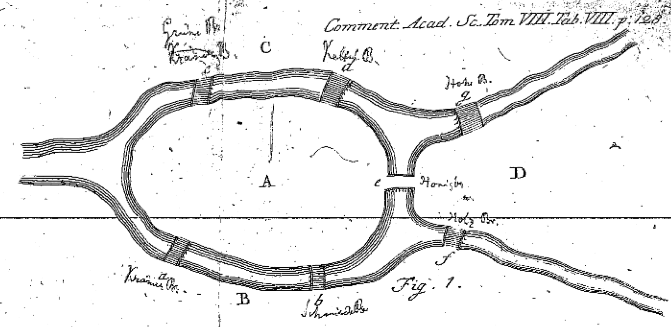
\includegraphics[width=10cm]{bridges.png}
\end{center}
\end{problem}

\begin{solution}
No, it is not possible. The drawing is equivalent to the following graph:
\begin{center}
\begin{tikzpicture}[very thick,edge from parent/.style={draw,<-},level/.style={sibling distance=30mm/#1}]
\draw (0, 0) node [vertex] (a) {$a$};
\draw (0, 3) node [vertex] (c) {$c$};
\draw (0, -3) node [vertex] (b) {$b$};
\draw (4, 0) node [vertex] (d) {$d$};
\path (a) edge [bend left] (c);
\path (c) edge [bend left] (a);
\path (a) edge [bend left] (b);
\path (b) edge [bend left] (a);
\draw (a) -- (d);
\draw (b) -- (d);
\draw (c) -- (d);
\end{tikzpicture}
\end{center}
The degrees of all vertices is odd, so no Euler circuit exists by the previous problem.
\end{solution}

\begin{problem} % 10
In connected graph $G$, every vertex has even degree. Suppose we began a walk at vertex $v$. We get stuck if we enter a vertex that has no outgoing edge
we haven't yet traversed. Show that it is impossible to get stuck at a vertex other than $v$, and use this fact to show that any connected graph $G$, with
all vertices having even degree, has an Euler circuit.
\end{problem}

\begin{solution}
We can't get stuck because every vertex has even degree. When we enter a vertex, we use up one edge, but since there are an odd number of edges remaining,
there must be at least one we can leave through. Therefore the walk must end at vertex $v$.

We use this fact to construct any circuit beginning and ending with $v$ for an arbitrary $v$. The graph that remains after removing all the edges in the first circuit
also has even degree, so we can simply repeat this process. We can combine multiple circuits to create one larger circuit.
\end{solution}

That concludes the Power Round. We hope you learned something cool!

\end{document}
